% Dies ist die Hauptdatei, von der aus das Gesamtdokument erzeugt wird.  Diese
% Datei sollten Sie zunächst umbenennen, damit sie keinen generischen Namen
% hat!  Dann wird sie mit LuaLaTeX kompiliert.

% In der Datei defs.tex werden alle globalen LaTeX-spezifischen Einstellungen
% vorgenommen
% Jede LaTeX-Datei beginnt mit der Dokumentenklasse.  Für diese Vorlage wurde
% die Klasse "scrreprt" von KOMA-Script gewählt, die in etwa der
% Standardklasse "report" entspricht, allerdings wesentlich mehr Möglichkeiten
% bietet und im gewissen "moderner" ist.  Eine sehr ausführliche Dokumentation
% zu KOMA-Script findet man unter der folgenden Adresse:
% http://mirrors.ctan.org/macros/latex/contrib/koma-script/doc/scrguide.pdf
\documentclass[
  % die Schriftgröße - sollten Sie nicht ändern
  fontsize=12pt,
  % das Papierformat, also DIN A4
  paper=A4,
  % Literaturverzeichnis ins Inhaltsverzeichnis
  bibliography=totoc,
  % andere Verzeichnisse ebenfalls ins Inhaltsverzeichnis
  listof=totoc,
  % abgesetzte Formeln linksbündig
  fleqn,
  % für die Satzspiegelkonstruktion - siehe KOMA-Doku
  DIV=12,
  % Bindekorrektur (linker Rand) - evtl. anpassen
  BCOR=1mm,
  % die im Text verwendeten Sprachen (u.a. für das Paket babel); die
  % letztgenannte (!) Sprache ist die Standardsprache; "n"german steht für die
  % neue Rechtschreibung
  english,ngerman,
  % weil (s.u.) das Paket geometr verwendet wird
  usegeometry,
  % wie Absätze gesetzt werden: ohne Einzug, halbe Zeile Abstand
  parskip=half-
]{scrreprt}

% Beschriftungen für Tabellen kommen linksbündig über die Tabelle
\KOMAoption{captions}{tableheading,nooneline}
\setcaptionalignment[figure]{c}
\setcaptionalignment[table]{l}

% wird für die Titelseite benötigt
\usepackage{geometry}

% Standardpaket für Lokalisation, siehe Option "ngerman" oben
\usepackage{babel}
% Laden von optimierten Trennmustern
\babelprovide[hyphenrules=ngerman-x-latest]{ngerman}

% Standardpaket für mathematische Zusatzfunktionen; wenn Sie keine
% mathematischen Formeln brauchen, können Sie diese Zeile löschen
\usepackage{amsmath}

% die Hauptschrift Libertinus
\usepackage{libertinus-otf}
% die "Schreibmaschinenschrift" Anonymous Pro, angepasst
\usepackage{AnonymousPro}
\setmonofont{AnonymousPro}[Scale=MatchLowercase,FakeStretch=0.85]

% etwas größerer Zeilenabstand als im Buchsatz
\linespread{1.1}

% Paket für Feinkorrekturen an der Typographie, das für ein ausgewogeneres
% Schriftbild sorgt
\usepackage{microtype}

% Paket für kontextsensitive Anführungszeichen
\usepackage{csquotes}
% Shortcut, damit aus dem eigentlich falschen Zeichen " richtige
% Anführungszeichen je nach Sprache werden
\MakeOuterQuote{"}

% Paket, das den Befehl \includegraphics ermöglicht
\usepackage{graphicx}

% komfortablere Aufzählungen als in Standard-LaTeX; ein Beispiel findet man in
% chap3.tex
\usepackage{enumitem}

% Paket für mehr als die üblichen Standardfarben
\usepackage[dvipsnames]{xcolor}
% Definition der "Hausfarben" der HAW
\definecolor{haw}{HTML}{003CA0}
\definecolor{haw2}{HTML}{0096D2}
\definecolor{haw3}{HTML}{A0BEDC}

% typographisch anspruchsvolle Tabellen; siehe chap3.tex
\usepackage{booktabs}

% zum Erstellen des Literaturverzeichnisses; der gängige Stil APA ist hier
% bereits eingestellt
\usepackage[style=apa]{biblatex}
% eine Beispieldatei für ein Literaturverzeichnis
\addbibresource{demo.bib}

% für die Erzeugung der Grafiken in chap3.tex; wenn Sie PGF/TikZ nicht
% verwenden wollen, können Sie diese Zeilen entfernen
\usepackage{tikz}
% Zusatzbibliotheken für TikZ, die in den genannten Beispielen verwendet
% werden
\usetikzlibrary{calc,intersections,angles,3d}

% für die Erzeugung des Codeblocks in chap3.tex; wenn in Ihrer Arbeit keine
% Codeblöcke vorkommen, können Sie diese Zeilen entfernen
\usepackage{listings}
% Anpassung des Erscheinungsbildes des Codeblocks; mehr dazu in der
% Dokumentation des Pakets "listings"
\lstdefinestyle{mystyle}{
    backgroundcolor=\color{gray!20},
    keywordstyle=\color{haw2},
    numberstyle=\footnotesize\color{haw},
    basicstyle=\ttfamily\small,
    captionpos=t,
    frame=single,
    framerule=0pt,
    keepspaces=true,
    numbers=left,
    numbersep=6pt,
    belowcaptionskip=1em,
    aboveskip=\bigskipamount,
}
\lstset{style=mystyle}
% damit es "Codeblock" und nicht "Listing" heißt
\renewcommand{\lstlistingname}{Codeblock}

% für die Verlinkung innerhalb des PDF-Dokuments, für PDF-Lesezeichen und
% PDF-Metadaten; dieses Paket sollte üblicherweise immer als letztes geladen
% werden
\usepackage[colorlinks=true,allcolors=haw,hyperfootnotes=false,pageanchor=true,linktoc=all]{hyperref}

% für die Druckversion können Sie die obige Zeile durch die folgende ersetzen,
% damit Links nicht blau dargestellt werden:
% \usepackage[draft]{hyperref}

% Metadaten des PDF-Dokumentes; setzen Sie hier Ihren eigenen Namen sowie den
% Titel Ihrer Arbeit ein
\hypersetup{pdfauthor={Prof. Dr. Edmund Weitz}}
\hypersetup{pdftitle={Handreichung zur Formatierung von Bachelorarbeiten}}


% Wenn das Kommentarzeichen entfernt wird, kann man mit einem Befehl wie
%
% \includeonly{chap2,chap3}
%
% erreichen, dass nur ausgewählte Dateien kompiliert werden.  Das ist für die
% Arbeit an umfangreichen Dokumenten hilfreich, weil es Zeit spart.  Für das
% Erstellen des fertigen Dokuments muss der Befehl natürlich wieder
% auskommentiert werden, damit alle Referenzen aktuell sind und die
% Seitenzahlen stimmen.

% Hier beginnt das eigentliche Dokument.  Sie können weitere Dateien
% hinzufügen und natürlich auch vorhandene weglassen.  Die vorhandene
% Dateistruktur ist lediglich als Beispiel gedacht.
\begin{document}
% In dieser Umgebung wird die Titelseite separat vom restlichen Text gesetzt
\begin{titlepage}
  % andere Seitenränder als im Rest der Arbeit
  \newgeometry{lmargin=2cm,tmargin=7mm,rmargin=5mm,bmargin=1cm}
  % die "Hausfarbe" der HAW; diese und die folgenden Einstellungen sind lokal
  % und gelten nur innerhalb der Umgebung "titlepage"
  \color{haw}
  % Blocksatz für die Titelseite deaktivieren
  \raggedright
  % Logo rechtsbündig setzen
  \hfill
\includegraphics[width=7cm]{HAW_Marke_RGB_300dpi}\\

  % vertikaler Abstand
  \vspace{5cm}

  % Wahl der "Hausschrift" Open Sans der HAW, die als Schrift auf Ihrem
  % Rechner installiert sein muss
  \setmainfont{Open Sans}
  % etwas kleiner als üblich
  \small
  % fett und in Majuskeln
  \textbf{BACHELORARBEIT}

  % vertikaler Abstand
  \vspace{8mm}

  % der Titel der Arbeit als "Seite in der Seite"; natürlich müssen Sie hier
  % Ihren Titel eintragen
  \begin{minipage}{0.8\linewidth}
    % Wahle der zweiten "Hausschrift" der HAW, die ebenfalls auf Ihrem Rechner
    % bereits vorhanden sein muss
    \setmainfont{Martel Heavy}
    % ziemlich große Schrift
    \LARGE
    % [1mm] steht jeweils für einen etwas größeren Durchschuss
    Handreichung\\[1mm]
    zur Formatierung\\[1mm]
    von Bachelorarbeiten\\[1mm]
    am Department Medientechnik\\
    % am Ende noch ein waagerechter Strich, das CD will es so...
    \,\rule{11mm}{1.2mm}
  \end{minipage}

  % vertikaler Abstand, überraschenderweise
  \vspace{1cm}

  % hier korrektes Datum und Ihren Namen eingeben
  vorgelegt am 26. März 2022\\
  Marlene Mustermann

  % letzter vertikaler Abstand für heute
  \vspace{5cm}

  % noch eine "Seite in der Seite", etwas nach rechts geschoben
  \hspace*{37mm}
  \begin{minipage}{0.5\linewidth}
    % Namen und Titel der beiden Prüfer eintragen
    \begin{tabular}{@{}ll}
      Erstprüferin: & Prof. Dr. Vera Musterfrau\\[-.3mm]
      Zweitprüfer: & Prof. Dr. Heinz Musterdorf \\
    \end{tabular}\\

    % noch ein horizontaler Strich
    \,\rule{9mm}{1mm}\\[1.5mm]

    \textbf{HOCHSCHULE FÜR ANGEWANDTE}\\
    \textbf{WISSENSCHAFTEN HAMBURG}\\
    Department Medientechnik\\
    Finkenau 35\\
    22081 Hamburg
  \end{minipage}
\end{titlepage}
% setzt die Geometrie wieder auf die Standardwerte zurück
\restoregeometry

% für die Seite mit dem Abstract keine Seitenzahl ausgeben
\thispagestyle{empty}

\section*{Zusammenfassung}

% Hier ersetzen Sie bitte die vorhandenen Texte durch Ihre eigenen
% Zusammenfassungen
Der Arbeit beginnt mit einer kurzen Beschreibung ihrer zentralen Inhalte, in
der die Thematik und die wesentlichen Resultate skizziert werden.  Diese
Beschreibung muss sowohl in deutscher als auch in englischer Sprache vorliegen
und sollte eine Länge von etwa 150 bis 250 Wörtern haben.  Beide Versionen
zusammen sollten nicht mehr als eine Seite umfassen.  Die Zusammenfassung
dient u.\,a.\ der inhaltlichen Verortung im Bibliothekskatalog.

% Zum Wechseln der Sprache siehe den Kommentar in chap3.tex
{
  \begin{otherlanguage}{english}
    \section*{Abstract}

    The thesis begins with a brief summary of its main contents, outlining the
    subject matter and the essential findings.  This summary must be provided
    in German and in English and should range from 150 to 250 words in length.
    Both versions combined should not comprise more than one page.  Among
    other things, the abstract is used for library classification.
  \end{otherlanguage}
}

% In der Titelei werden römische Ziffern für die Seitenzahlen verwendet;
% gleichzeitig wird durch diesen Befehl die aktuelle Seitenzahl auf eins
% gesetzt
\pagenumbering{Roman}

% Inhaltsverzeichnis
\tableofcontents

% Abbildungsverzeichnis, kann evtl. weggelassen werden
\listoffigures

% Tabellenverzeichnis, kann evtl. weggelassen werden
\listoftables

% weitere Verzeichnisse (z.B. Codeblöcke) sind theoretisch möglich

% neue Seite, vorsichtshalber
\clearpage
% ab jetzt arabische Ziffern und wieder auf eins setzen
\pagenumbering{arabic}
\section{Einleitung}\label{sec:einleitung}
dasd \cite[]{chai_optimizing_2024}
\chapter{Vorgehensweise} 
Im folgenden Kapitel beschäftige ich mich mit der Ausarbeitung theoretischer Grundlagen als auch mit der groben Planung des Algorithmus und deren Komponenten.
\section{Überblick zum genetischen Algorithmus}
Genetische Algorithmen versuchen die Prozesse der natürlichen Evolution nachzuahmen. Dabei wird initial eine Population von möglichst unterschiedlichen Individuen erstellt, hier eine Konfiguration aus Hyperparameter, die dann durch die Fitness-Funktion bewertet wird. Ein niedriger Wert bei der Fitnessfunktion bedeutet eine gute Lösung. Mittels einer Selektion werden schlechtere Konfigurationen entfernt, sodass durch eine Kombination mehrerer guter Lösungen wieder bessere entstehen können. Um eine große Diversität zu gewährleisten, werden die einzelnen Individuen mutiert, dabei werden einzelne Merkmale arithmetisch verschoben. Dieser Prozess wiederholt sich ständig, sodass weitere, womöglich bessere, Konfiguration entdeckt werden.
\tikzstyle{block} = [rectangle, draw, text width=10em, text centered, rounded corners, minimum height=3em]
\begin{figure}[h]
	\centering
	\begin{tikzpicture}
		[node distance=1.8cm,
		start chain=going below,]
		\node (n1) at (0,0) [block]  {Selektion};
		\node (n2) [block, below of=n1] {Rekombination};
		\node (n3) [block, below of=n2] {Mutation};
		\node (n4) [block, below of=n3] {Berechnung Fitness};
		\node (n5) [block, left of=n4, node distance=2in] {Start:\\Population erzeugen};
		% Connectors
		\draw [->] (n1) -- (n2);
		\draw [->] (n2) -- (n3);
		\draw [->] (n3) -- (n4);
		\draw [->] (n5) -- (n4);
		\draw [->] (n4.east) -| ++(1,0) |- (n1.east);
	\end{tikzpicture}
	\caption{Grundschema Genetischer Algorithmus \parencite[Seite 5]{stelldinger_naturanaloge_2024}}
\end{figure}
\section{Überblick Neuronale Netze}
Neuronale Netze sind eine Form des überwachten Lernens, das heißt sie lernen anhand von bereits bekannten Zielwerten. Im Beispiel der Klassifikation von Tierbildern ist beim überwachten Lernen bereits für jedes Bild bekannt, um welches Tier es sich dabei handelt. Das neuronale Netz erkennt selbstständig Muster in den Tierbildern, welche dann zur Generalisierung unbekannter Daten verwendet werden. Ziel hierbei ist die Extraktion der wichtigen Merkmale, nicht das stupide Auswendiglernen der Daten (\textit{"Overfitting"}). Das neuronale Netz wird dabei mit Trainingsdaten gefüttert, anhand dessen die Muster gelernt werden. Üblicherweise wird die Effektivität oder Genauigkeit des Modells an Daten überprüft, die nicht zum Training gehören \parencite{sonnet_neuronale_2022}.
\subsection{Hyperparameter in neuronalen Netzen}
Hyperparameter sind Parameter, welche den Lernprozess betreffen. Im Kontrast zu den Modellparametern, die während des Trainings aufgebaut werden, sind Hyperparameter beim Training bereits bekannt. Es gibt viele neuronale Netze, die Erfolg mit dynamischen Parametern haben \parencite{schaul_no_2013}. Andere typische Hyperparameter eines neuronalen Netzes beinhalten die Batch-Größe, Anzahl von Epochen sowie auch die Anzahl von Neuronen in der verdeckten Schicht. In dieser Hausarbeit beschränke ich mich auf die genannten Parameter.
\section{Aufbau des Genetischen Algorithmus}
Im nachfolgenden Kapitel beschäftige ich mich mit der Planung des genetischen Algorithmus, dabei wird auf die einzelnen Operationen eingegangen.
\subsection{Chromosom}
Ein Chromosome wird üblicherweise in binärer Darstellung kodiert. Dies hat den Vorteil, dass bitweise Operationen sehr effizient und schnell umsetzbar sind. Allerdings kann dies auch zu Problemen führen. Bei der Mutation oder Rekombination ist es daher zu beachten, dass die höherwertigen Bits (MSB) einer Zahl, die Zahl stärker verändern können als es die Least Significant Bits. Um diese Nicht-Linearität zu vermeiden, müssen die Operationen besser angepasst werden \parencite{herrera_tackling_1998}.  

Ein Chromosom besteht aus vier Parametern: Batch-Größe,  Neuronen in der verdeckten Schicht, Anzahl von Epochen und der Lernrate. Da die geplante Rekombination mit Operationen auf reellen und natürlichen Zahlen durchführt werden soll, habe ich mich gegen eine Repräsentation in Binärform entschieden. Bis auf die Lernrate werden alle Parameter als natürliche Zahl kodiert.
\subsection{Population}
Initial wird eine Startpopulation erzeugt, dabei wird aus einen vorher definierten Bereich zufällig eine Zahl gewählt.
\begin{itemize}
	\item \textbf{Lern Rate}: Es wird eine logarithmische Verteilung im Wertebereich von \(\left[ 0.1, 0.00001 \right]\) vorgenommen. Eine nicht-logarithmische Verteilung ist hierbei nicht gewünscht, da die Lernrate ansonsten in aller Regel sehr nah an \textit{0.1} bleibt. Eine logarithmische Verteilung garantiert hier eine ausgeglichene Verteilung.
	\item \textbf{Batch-Größe}: Stetige Gleichverteilung im natürlichen Intervall \(\left[ 8, 512 \right]\). 
	\item \textbf{Epochen}: Stetige Gleichverteilung im natürlichen Intervall \(\left[ 5, 20 \right]\). 
	\item \textbf{Neuronen in der verdeckten Schicht}: Stetige Gleichverteilung im natürlichen Intervall \(\left[ 10, 1000 \right]\). 
\end{itemize}
Durch erste Tests konnte eine maximale Konfiguration mit einer Batch-Größe von 512 und 1000 Neuronen in der verdeckten Schicht ermittelt werden. Eine größere Konfiguration ist mit der aktuell verwendeten Hardware nicht möglich, da der Grafikspeicher nicht ausreichend groß ist.

\subsection{Fitness}
Die Fitness bewertet eine mögliche Konfiguration an Hyperparameter innerhalb des neuronalen Netzes. Hierfür wird das neuronale Netz mit Daten trainiert und anschließend mit ungesehenen Daten validiert. Die Fehlerfunktion ("Loss"), auf Basis der Validierungsdaten, ist dabei ein wertvoller Indikator für ein gut trainiertes Netz, denn anders als die Genauigkeit, welche nur ein metrischer Wert ist, reflektiert die Fehlerfunktion auch bei kleinen Änderungen im Netz einen niedrigeren Wert. Daher gilt es diese Funktion zu minimieren \parencite[Kapitel~4.3]{goodfellow_deep_2016}. Insgesamt ist die Berechnung der Fitness ein sehr aufwändiges Unterfangen, da hierzu das komplette Netz trainiert und anschließend mit Validierungsdaten überprüft werden muss. Gemittelt dauert eine Berechnung eine Minute.

\subsection{Rekombination}
Die Rekombination erfolgt über zwei Elternteile. Hierfür wird im Wertebereich des Parameters eine Normalverteilung zwischen den zwei Elternteilen formiert. So ist ein Wert innerhalb der beiden Elternteile wahrscheinlich, nicht aber zwangsläufig verpflichtend. Durch einen Parameter kann die Standardabweichung beeinflusst werden. So kann ein Fokus entweder auf Exploitation oder Exploration gelegt werden. Diese Art von Rekombination ist inspiriert durch die Gauss-Mutation \parencite[Seite~8]{kruse_evolutionare_2013}. 
\begin{figure}[h]
	\centering
	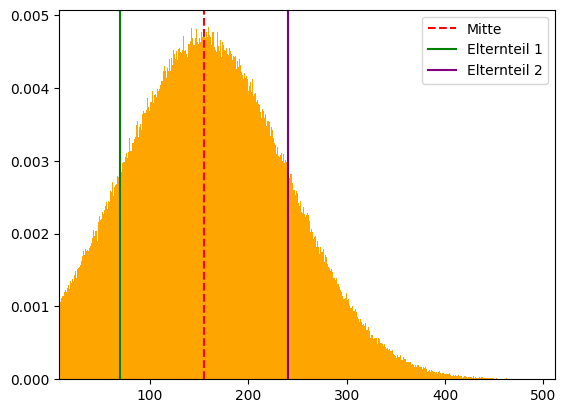
\includegraphics[width=1\linewidth]{rekombination.png}
	\caption{Normalverteilung bei der Rekombination für Batch-Größe}
	\label{fig:enter-label}
\end{figure}

\subsection{Selektion}
Die Selektion reduziert die Population nach der gewählten Strategie. So wird Platz für besser angepasste Individuen. Um bereits gefundene lokale Optimas nicht zu verlieren, werden pro Generation jeweils zwei Elitisten bestimmt, diese werden unverändert in die nächste Generation übernommen. Zusätzlich findet eine Turnierselektion zwischen zwei Chromosomen statt. Die Gewinner kommen in die nächste Generation, ein erneutes Auswählen findet nicht statt. So können auch schlechtere Chromosomen in die nächste Generation kommen, sodass lokale Optimas besser umgangen werden können. Durch die Turnierselektion wird die Population um 50\% reduziert.

\subsection{Mutation}
Die Mutation wird nach der Rekombination für jedes Konfiguration durchgeführt, die kein Elitist ist. Sie sorgt dafür, dass sich schlechtere wie auch bessere Konfigurationen verbessern oder verschlechtern können und sorgt für eine Diversität in der Population. Im genetischen Algorithmus wird jedes Gen mit einer Wahrscheinlichkeit von 20\% komplett neu generiert. So wird die Exploration verstärkt. 
\section{Bemerkungen zum Ansatz}
Der hier gewählte Ansatz hat seine Tücken. So ist die Wahl der Standardabweichung bei der Rekombination sehr wichtig, um eine Balance zwischen Exploration und Exploitation zu finden. In der Rekombination wird eher Wert auf die Exploitation gesetzt, während in der Mutation der Fokus auf die Exploration des Suchraums gesetzt wird. 
\chapter{Methodik}
\section{Datengrundlage des neuronalen Netzes}
\section{Startparameter für genetischen Algorithmus}
\section{Durchführung}
\section{Herausforderungen}
\section{Bewertung}
\chapter{Ergebnisse}
\section{Überblick}
Der genetische Algorithmus wurde mit einer Populationsgröße von 50 über 30 Generationen hinweg optimiert. Dabei konnte sowohl die Genauigkeit minimal verbessert werden als auch die Fehler reduziert. Der genetische Algorithmus konvergiert sehr schnell zum Ergebnis. Die Ausführung dauerte 14 Stunden. Dabei handelte es sich um die Konfiguration mit einer einer geringeren Standardabweichung bei der Rekombination, das bedeutet, dieser Lauf fokussierte sich mehr auf die Exploitation. Im Anhang finden sich die Resultate zum Lauf der Exploration.

\begin{figure}[h]
	\centering
	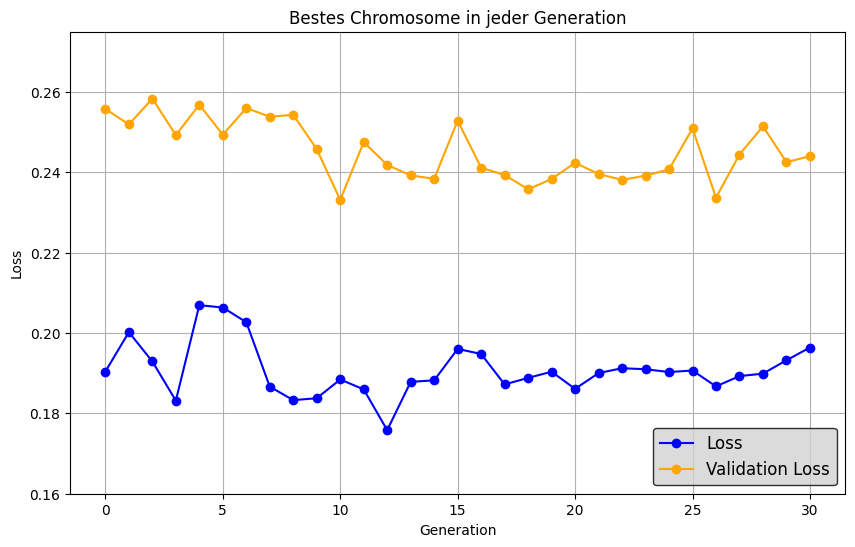
\includegraphics[width=1\linewidth]{loss.png}
	\caption{Geringster Fehler pro Generation}
	\label{fig:enter-label}
\end{figure}


\section{Interpretation der Ergebnisse}
Die Testergebnisse sind nicht wirklich aussagekräftig, denn die Fitness-Berechnung ist leider nicht deterministisch. So kann es passieren, dass ein Elitist, der gerade noch einen Fehler von 0.24 hatte, in der nächsten Generation einen Fehler von 0.23 ermittelt. Die Startkonfiguration der Neuronen sind zufällig und so fließt leider auch eine gewisse nicht-deterministische Komponente in die Fitness-Funktion ein. Dies wurde deutlicher, wenn probiert wurde, das beste Individuum zu reproduzieren: hierbei wurde oft ein schlechterer Wert erreicht. Das gute Ergebnis kam daher durch einen optimaleren Bias im Neuron.

Insgesamt konnte das Netz nicht merklich verbessert werden, dies könnte an der geringen Auswahl der Hyperparameter liegen. Wahrscheinlich wäre es besser ein tieferes Netz mit mehr Schichten zu nehmen, in welcher dann auch die Neuronenanzahl optimiert werden, dies würde aber auch den Suchraum extrem erweitern. Karlupia et. al. hatten Erfolge bei der Benutzung eines genetischen Algorithmus zur Optimierung eines CNN für die Gesichtserkennung. CNN's haben durch die Faltungs- und Pooling-Schichten deutlich mehr Hyperparameter zum Optimieren. \parencite{karlupia_genetic_2023}. 

Das rein zufällige Erstellen der Generationen nach "Random Grid Search", führt daher zu einen ähnlichen Ergebnis. Es liegt also nahe, dass die Optimierung der vier Hyperparameter schlicht weg zu wenig war. Die Devianz der einzelne Läufe waren dafür zu hoch.

\section{Verbesserungsmöglichkeiten}
Eine Erhöhung der Gene im Chromosom führt zu einem erweiterten Suchraum und mehr Dimensionen, so würde der Unterschied zu Grid Search, welches öfters Probleme mit einer hohen Anzahl von Dimensionen hat, größer werden. Daher erscheint es sinnvoll mehr Hyperparameter aufzunehmen. 

\section{Vergleich zu Grid Search}
Um einen Vergleich zu einer anderen Hyperparameter-Optimierungen bekommen wurde das gleiche neuronale Netz mittels Grid Search optimiert. Hierfür wurden die einzelnen Parameter im gleichen Intervall rasterförmig verstreut und ausprobiert. Dabei wurden um die 700 Kombinationen der Parameter ausgeführt und deren Genauigkeit/Fehler verglichen. Dabei wurde beobachtet, dass diese Brute Force Herangehensweise bei einem solch kleinen Netz zu ähnlich guter Konfiguration führt. 

\section{Fazit}
Genetische Algorithmen erweisen gute Dienste bei dem Optimierungsproblem, allerdings sollte drauf geachtet werden den Suchraum nicht zu klein zu lassen. Wenn es die Problemstellung zulässt, dann sollte am besten der Suchraum erst ausreichend groß skaliert werden. Wenn dann in gegebener Zeit keine gute Lösung gefunden wird, dann kann der Suchraum auch verkleinert werden. 

\chapter{Diskussion}
% -*- coding: utf-8 -*-

% Ausgabe des Literaturverzeichnisses; ohne weitere Optionen werden nur die
% Bücher und Artikel ausgegeben, die in der Arbeit auch zitiert werden.
\printbibliography

% markiert den Anfang des Anhangs
\appendix

% ein Kapitel, das nicht numeriert, aber trotzdem ins Inhaltsverzeichnis
% aufgenommen wird
\clearpage
\section*{Anhang}
\begin{figure}[p]
	\centering
	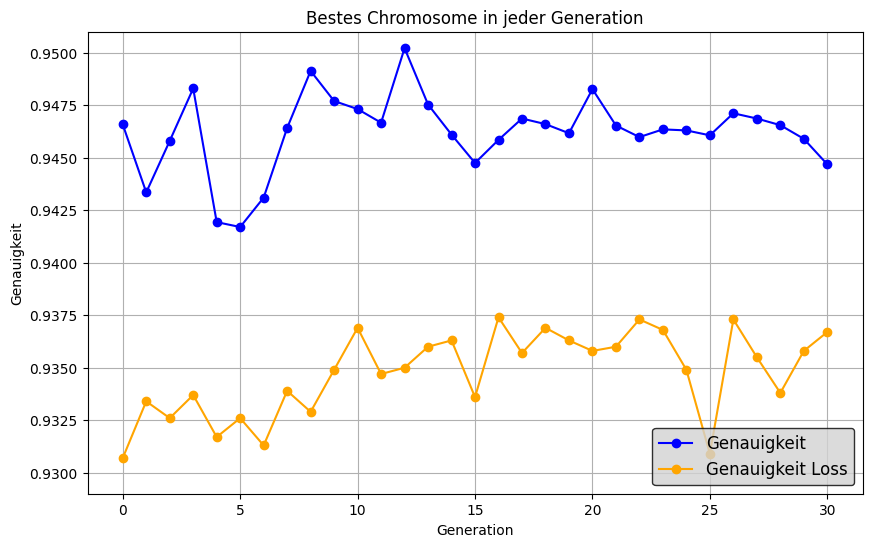
\includegraphics[width=1\linewidth]{acc.png}
	\caption{Lauf mit Priorisierung der Exploitation: Höchste Genauigkeit pro Generation}
	\label{fig:enter-label}
\end{figure}

\begin{figure}[p]
	\centering
	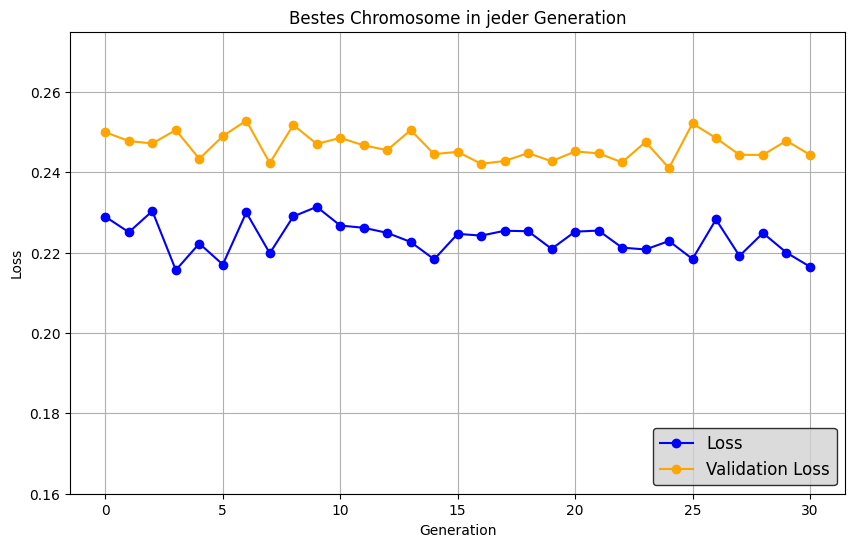
\includegraphics[width=1\linewidth]{loss_explore.png}
	\caption{Lauf mit Priorisierung der Exploration: Geringster Fehler pro Generation}
	\label{fig:enter-label}
\end{figure}

\begin{figure}[p]
	\centering
	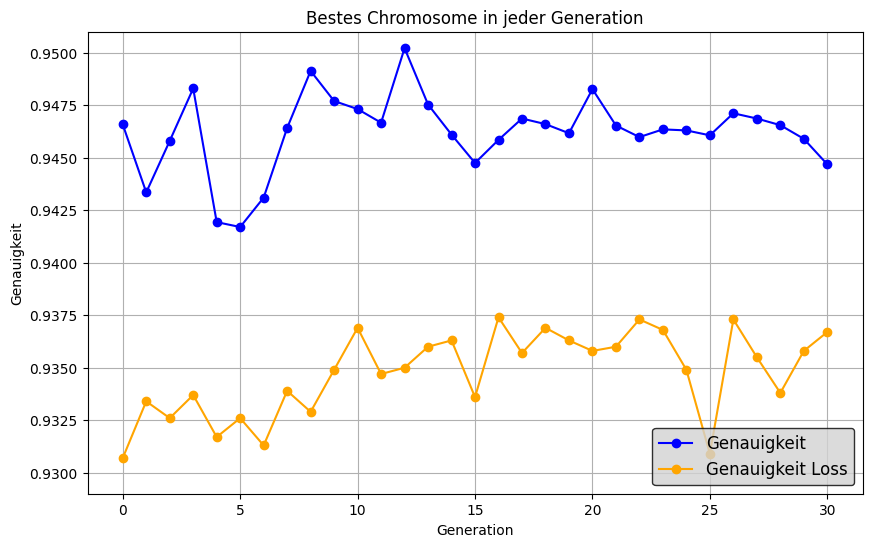
\includegraphics[width=1\linewidth]{acc.png}
	\caption{Lauf mit Priorisierung der Exploration: Höchste Genauigkeit pro Generation}
	\label{fig:enter-label}
\end{figure}


Der Sourcecode steht auf Github zur Verfügung:\\
\url{https://github.com/jonasmetzger2000/KI-STG-GI-Neural-Network-Optimizer}

% neue Seite
\clearpage

% keine Seitenzahl
\thispagestyle{empty}

% keine Nummerierung, keine Aufnahme ins Inhaltsverzeichnis
\section*{Eigenständigkeitserklärung}

% Hier müssen Sie natürlich den Titel der Arbeit sowie Ort und Datum ersetzen:
Hiermit versichere ich, dass ich die vorliegende Bachelorarbeit mit dem Titel
\begin{center}
  \textbf{Optimierung der Hyperparameter eines Neuronalen Netzes durch einen evolutionären Algorithmus}
\end{center}
selbstständig und nur mit den angegebenen Hilfsmitteln verfasst habe.  Alle
Passagen, die ich wörtlich aus der Literatur oder aus anderen Quellen wie
z.\,B. Internetseiten übernommen habe, habe ich deutlich als Zitat mit Angabe
der Quelle kenntlich gemacht.

\vspace{2cm}

Hamburg, 2. August 2024

\end{document}